% DRAFT / AUTHORITY0 / NO_RESULT / NOT_FOR_SUBMISSION
% ICASSP 2027 official-template migration. Author metadata remains pending.
\pdfminorversion=7
\documentclass{article}
\usepackage{spconf,amsmath,amssymb,booktabs,array,balance,graphicx,microtype,xcolor}
\usepackage[T1]{fontenc}
\usepackage[hidelinks]{hyperref}

\definecolor{holdred}{RGB}{160,22,22}
\newcommand{\DraftState}{\textcolor{holdred}{\textbf{DRAFT / AUTHORITY0 / NO\_RESULT / NOT\_FOR\_SUBMISSION}}}
\newcommand{\ResultHold}{\textcolor{holdred}{\textsf{HOLD}}}
\newcommand{\K}{K}

\title{PhaseSet: Permutation-Invariant Periodic Relation Tokens\\
for Multi-Person Motion--Language Retrieval}
\name{Author metadata pending --- NOT FOR SUBMISSION}
\address{Affiliation metadata pending\\\DraftState}

\begin{document}
\ninept
\maketitle
\begin{center}
\fbox{\parbox{0.93\linewidth}{\centering
This manuscript registers a method and evaluation protocol only. No training run,
test score, confidence interval, or submission authority is represented.}}
\end{center}

\begin{abstract}
Group motions can share actor marginals and the same multiset of pair relations
while differing in which relations meet at each actor. We register PhaseSet, a
permutation-invariant residual for bidirectional multi-person motion--language
retrieval. Six fixed Morlet bands produce directed pair descriptors; symmetric
pair statistics and actor--relation incidence moments yield six group tokens.
The topology branch is exactly zero at two actors, and all edges are processed
with deterministic streamed reductions. The confirmatory protocol fixes a
572-capture Embody 3D eligibility census, a participant-component-disjoint
400/96/76 split, unseen-cardinality $K{=}3$ testing, 33 training attempts,
eight hypotheses, one sealed test, and 100,000 clustered bootstrap draws. This
is a \textbf{NO\_RESULT} technical draft: every empirical cell is held.
\end{abstract}

\begin{keywords}
multi-person motion, text--motion retrieval, periodic relations, set representation
\end{keywords}

\section{Problem and claim boundary}
Single-person retrieval already includes contrastive motion synthesis and
fine-grained wavelet encoders \cite{tmr2023,wamo2026}. Dyadic motion work covers
interaction-aware retrieval and frequency-guided editing
\cite{mime2026,interedit2026}. Multi-person language systems cover open-domain
generation and instruction-based understanding
\cite{multimotion2024,socialgen2025,llammo2026}. Periodic video-language
reasoning also appears in action counting \cite{countllm2025}. Consequently,
PhaseSet makes no broad ``first'' claim for motion--language, frequency-aware
retrieval, or multi-human understanding.

The sole registered question is narrower: \emph{does frequency-specific
actor--relation incidence structure add retrieval utility beyond a qualified
group encoder and seven matched structural controls?} The contribution is a
fixed specification plus a fail-closed experiment. It is not generation,
editing, causal phase inference, role recognition, or an official
reimplementation of another model. Language supplies semantic retrieval tokens
but cannot generate, select, edit, or supervise physical phase, lag, power, or
coherence fields.

\begin{figure*}[t]
\centering
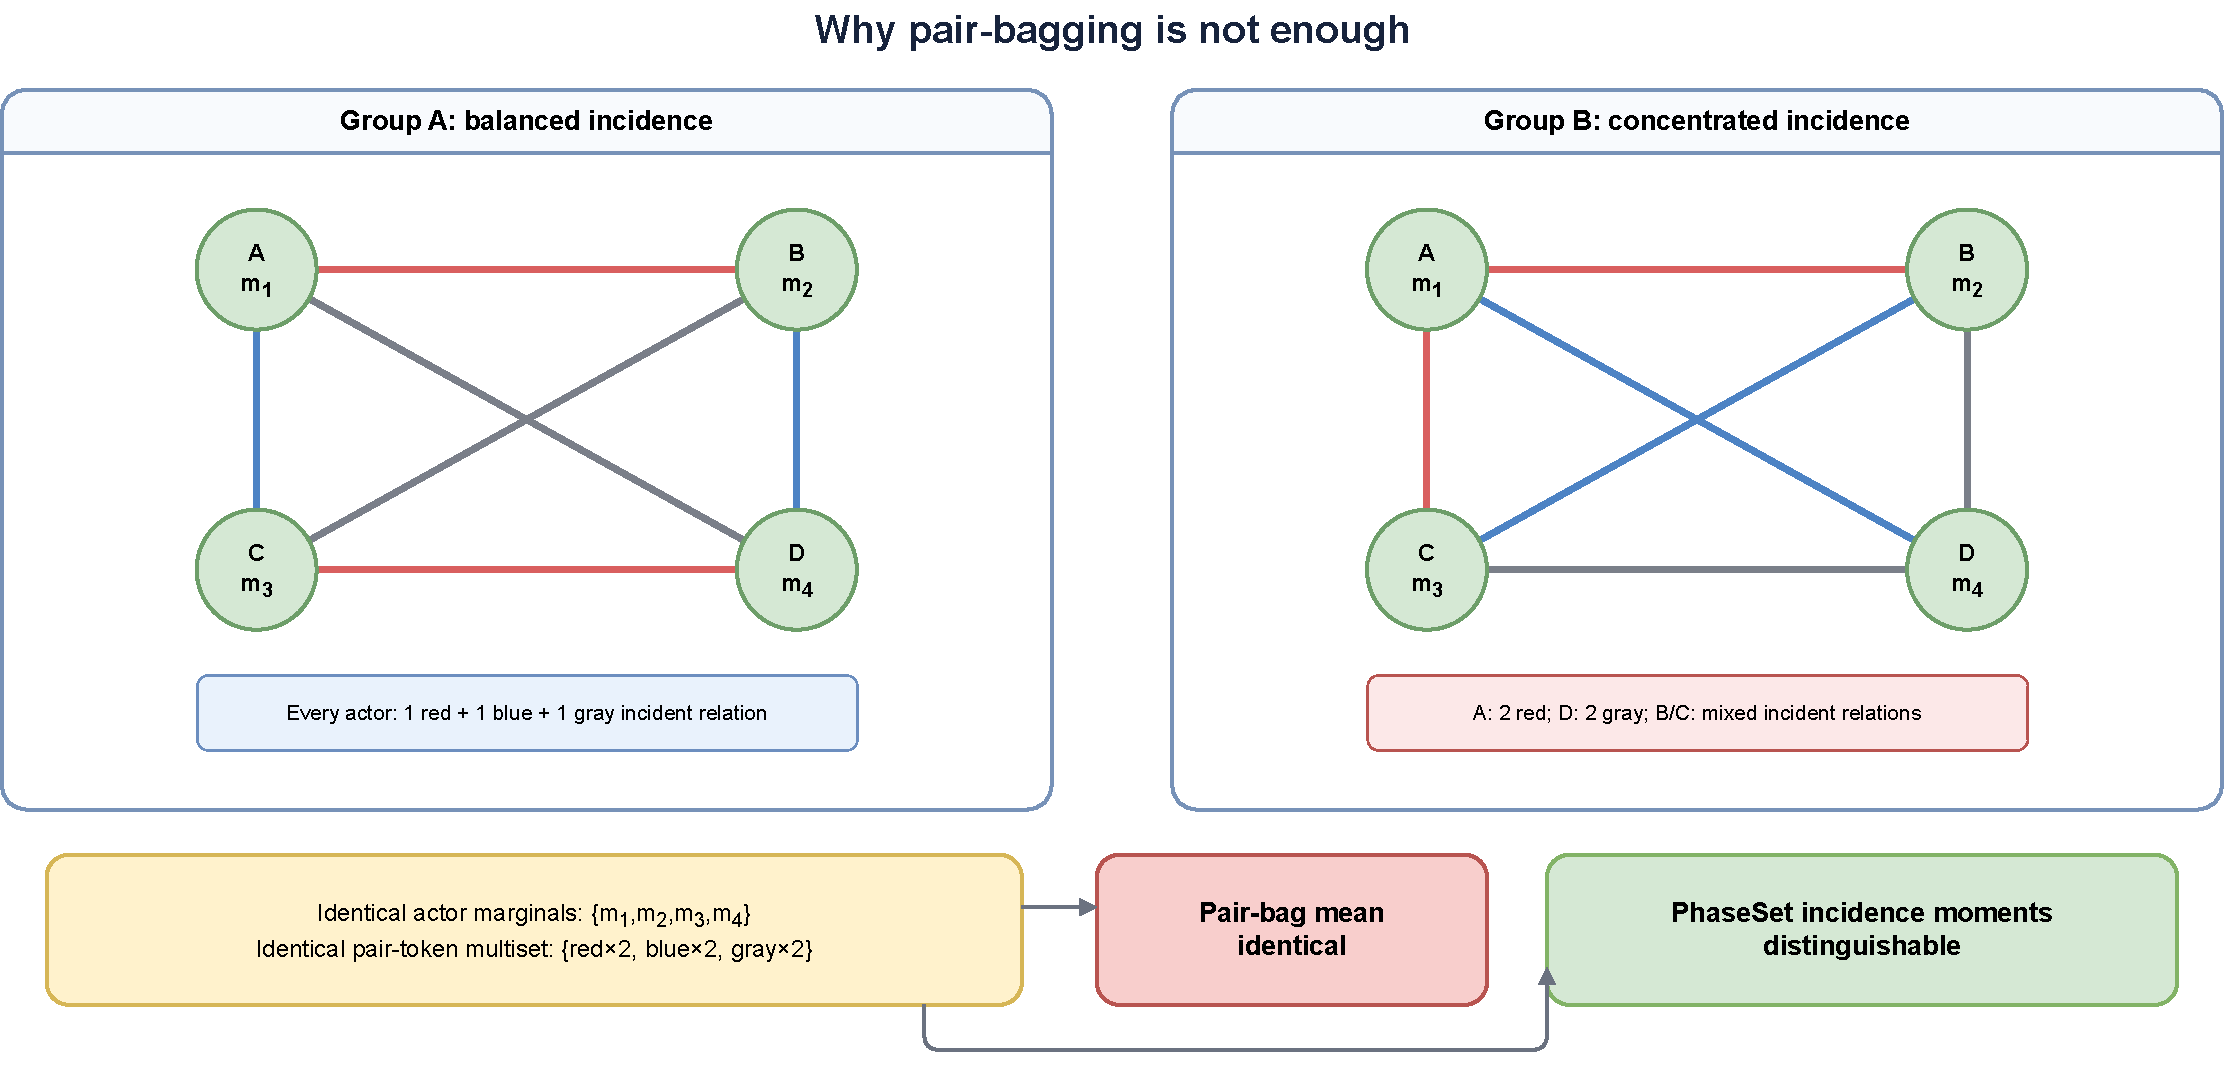
\includegraphics[width=0.95\textwidth]{../figures/phaseset_motivation.pdf}
\caption{Conceptual counterexample (not data or a result). Actor marginals and
the pair-token multiset are identical, so pair-bag averaging cannot distinguish
the groups; incident relation moments retain their different ownership.}
\label{fig:motivation}
\end{figure*}

\section{Related evidence}
Embody 3D provides synchronized multi-person motion, audio, and text at a
larger official scale than the eligibility subset used here
\cite{embody3d2025}. Multi-TPC offers natural triadic conversation, whereas
M3Act3D offers synthetic large-$K$ group activity; we reserve them for
cross-domain and engineering probes, respectively
\cite{multitpc2026,m3act2024}. Neither is confirmatory evidence for the present
retrieval claim. SocialGen/SocialX and Multi-Motion support variable-person
modeling, but their autoregressive/generative tasks and constructed data do not
replace native full-gallery retrieval \cite{socialgen2025,multimotion2024}.

The five supplied reference papers further delimit the task. MotionMaster is
single-person generation/editing; LangPose uses language as a pose-lifting
pretraining prior; HMVLM is a single-person multi-task language model; and
Pose2Lang3D distills 3D cues into static 2D-pose VQA
\cite{motionmaster2026,langpose2026,hmvlm2025,pose2lang3d2026}. They motivate
lineage, masking, task-interference, and privileged-information audits, not a
PhaseSet result. Cross-wavelet analysis itself is longstanding
\cite{grinsted2004}; our fixed descriptors are pooled motion features, not
novel signal-processing estimators.

\section{PhaseSet}
\subsection{Input and deterministic periodic relations}
An input is a dynamically padded tensor of $K\!\geq\!2$ actors, 200 frames,
and 22 body joints, with actor/joint/frame masks. A shared 512D actor encoder
uses no actor ID. Motion is resampled to 20 Hz; an independently hashed 20-Hz
Morlet bank retains PhasePair's six physical center frequencies while its
legacy 30-Hz tap bytes remain unchanged. Each response is computed once per actor. For every
valid unordered pair $\{i,j\}$ and band $b$, the inherited directed 13D
descriptor $d_b(i{\to}j)$ contains log auto-powers for the ordered endpoints,
coherence-like magnitude, cosine/sine of principal relative phase, wrapped
delay, a signed-phase-valid bit, and a six-way band indicator. These are
motion-derived descriptors, not causal or physical measurements.

All pairs are visited lexicographically in canonical 64-edge microblocks. The
implementation allocates no tensor with two actor axes. Pair processing is
$O(K^2)$ but streamed; if all exact edges exceed the frozen resource envelope,
the API returns \texttt{RESOURCE\_LIMIT} instead of dropping actors or sampling
edges.

\subsection{Pair and incidence paths}
A shared half-edge network and a symmetric pair network compute
\begin{equation}
\begin{split}
u_{ij}^{b}&=H(d_b(i{\to}j)),\quad u_{ji}^{b}=H(d_b(j{\to}i)),\\
p_{ij}^{b}&=P\!\left(u_{ij}^{b}+u_{ji}^{b},
 |u_{ij}^{b}-u_{ji}^{b}|,u_{ij}^{b}\odot u_{ji}^{b}\right).
\end{split}
\label{eq:pair}
\end{equation}
Ordered concatenation is prohibited. The pair component $\bar p_b$ is the
canonical masked mean over $p_{ij}^{b}$. For actor $i$, incident half-edges
produce mean offset from the band-global mean, population second central
moment $M2$, coverage $\deg(i)/(K-1)$, and missingness. The topology NodeMLP
input is exactly $[\Delta\mathrm{mean},M2,\mathrm{coverage},\mathrm{missing}]$.
A node is valid only at degree at least two; the post-MLP hard gate has no
biased layer after it. Thus at $K{=}2$ the topology residual and its parameter
gradients are exact positive zero.

\begin{figure*}[t]
\centering
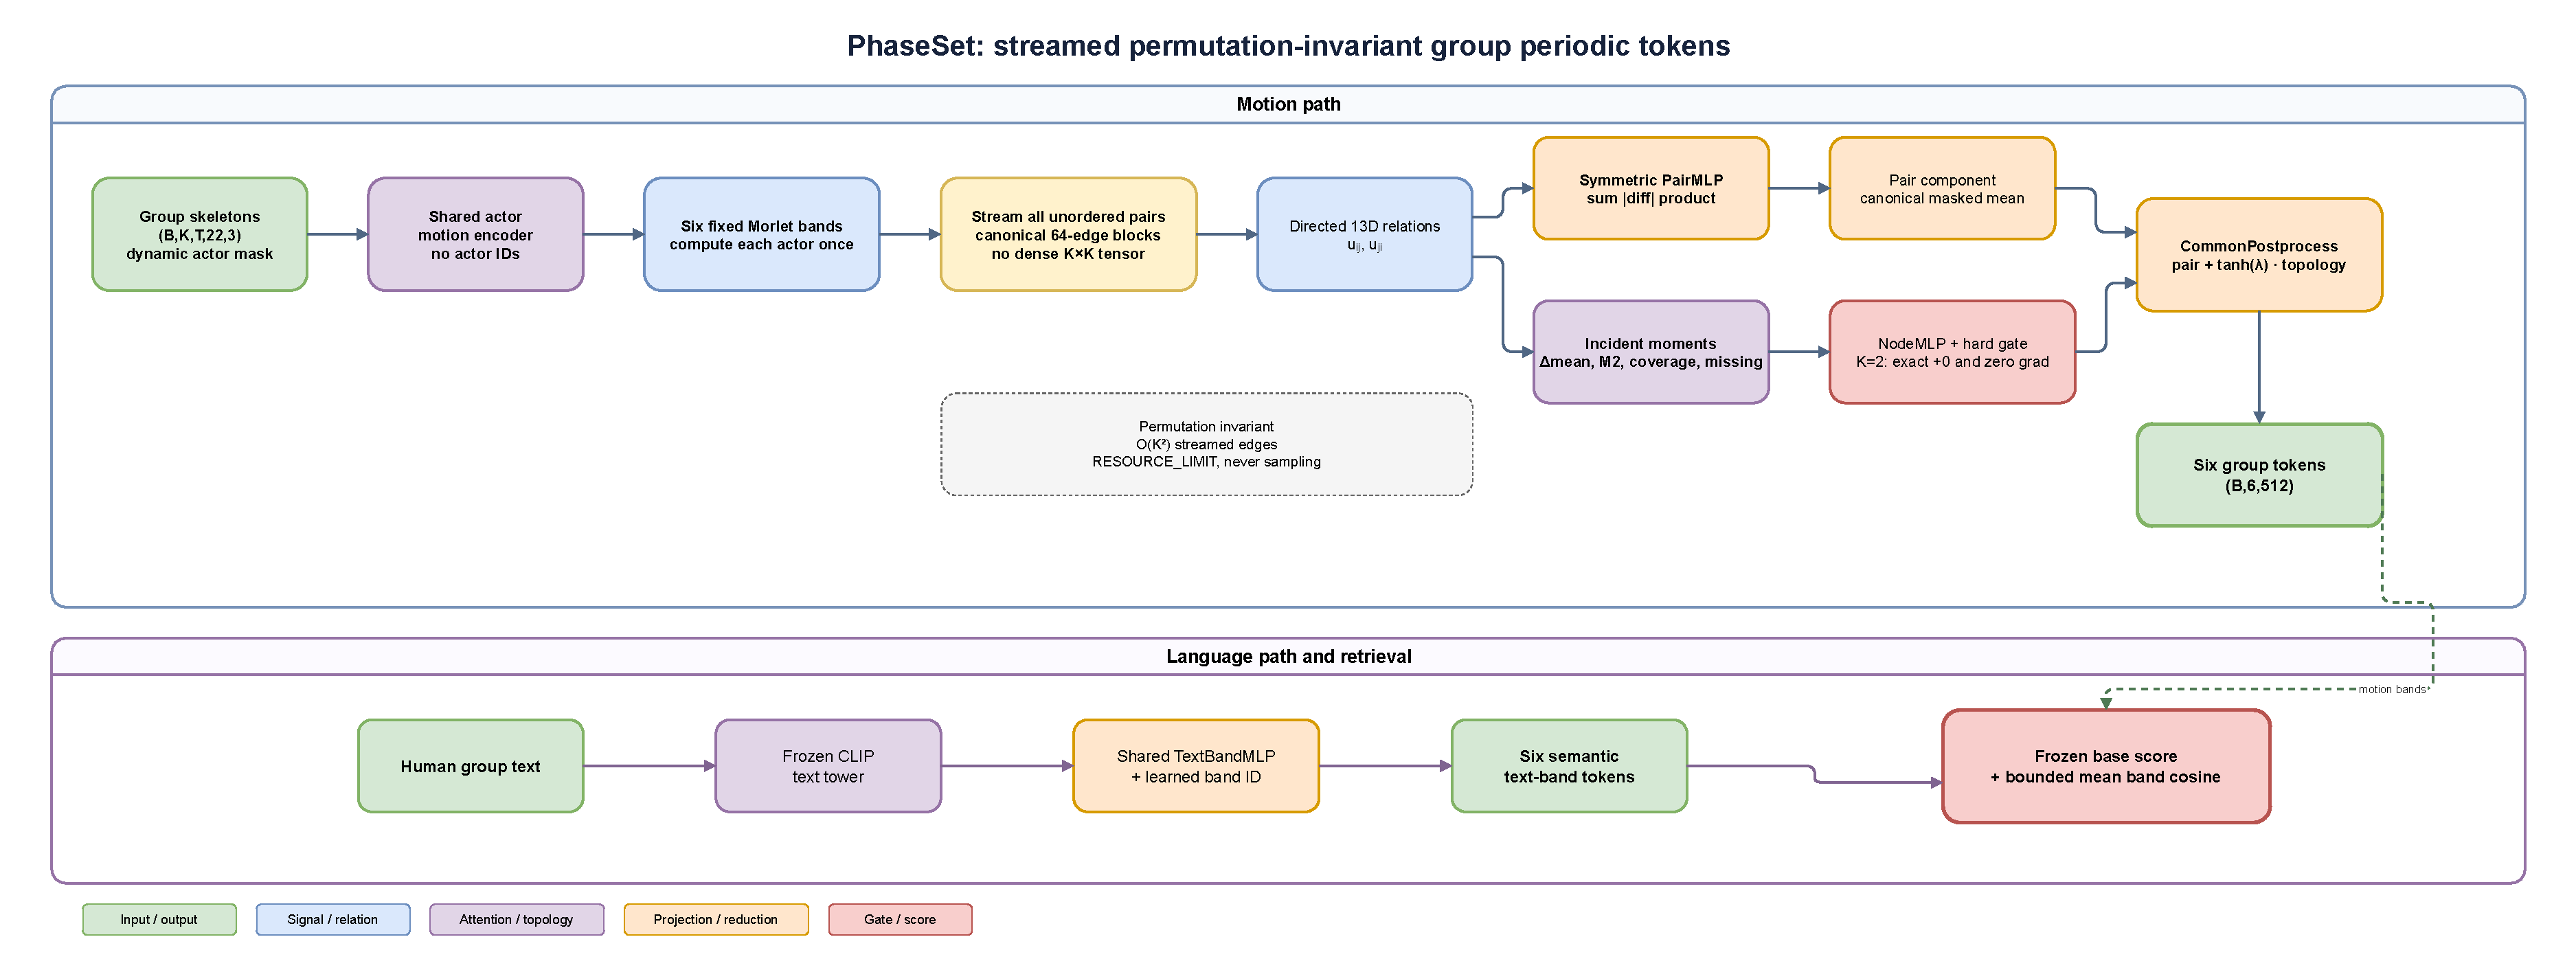
\includegraphics[width=0.96\textwidth]{../figures/phaseset_architecture.pdf}
\caption{Registered architecture (conceptual, no-result). Directed relations
feed a symmetric pair mean and incident-moment topology path; a hard $K{=}2$
gate preserves dyadic equivalence. Six motion tokens align with six semantic
text-band tokens on top of the frozen qualified base score.}
\label{fig:architecture}
\end{figure*}

Let $q_b$ be the canonical masked mean of valid node outputs. The band token is
\begin{equation}
g_b=m_b\,C\!\left(\bar p_b+\tanh(\lambda_b)q_b\right),
\label{eq:token}
\end{equation}
where $m_b$ is the band-valid mask and $C_b$ is the common postprocessor. The
capacity-matched pair-only control passes exact positive zero for $q_b$ through
the same $C_b$. Fixed-tree float64 microblock reduction, compensated
microblock accumulation, and fixed-order Chan merges make the output invariant
to registered chunk sizes.

\subsection{Text alignment and objective}
CLIP's frozen text encoder supplies an embedding \cite{clip2021}. A shared
TextBandMLP and learned band ID yield text tokens $\ell_b$. For capture $x$ and text $y$,
\begin{equation}
S(x,y)=S_{\mathrm{base}}(x,y)+\tanh(\alpha)
\frac{\sum_b m_b\cos(g_b,\ell_b)}{\sum_b m_b}.
\label{eq:score}
\end{equation}
The externally supplied base scores are frozen. Variable-positive symmetric
InfoNCE treats every registered caption for one capture as positive; windows or
captions never become independent statistical units.

\section{Frozen data protocol}
The primary source is native multi-person Embody 3D, subject to its access and
non-redistribution terms \cite{embody3d2025}. The project-registered,
public-safe eligibility census has 572 captures, 69 participants, 20.673 scene
hours, and 16 participant co-occurrence components: 27 captures have $K{=}3$
and 545 have $K{=}4$. The split is 400 train / 96 validation / 76 test captures
and 48/10/11 participants, with neither participant nor capture overlap.
Crucially, \emph{all} 27 $K{=}3$ captures are in test; $K{=}3$ is therefore an
unseen-participant and unseen-cardinality slice. We must not imply that
training saw $K{=}3$.

Motion uses 22 SMPL-X body joints, antialiased 30-to-20 fps resampling, and
nonoverlapping 10 s (200-frame) windows. The common origin is the first valid
frame's all-group pelvis centroid; centering/orienting around an indexed actor
is forbidden. Whole-group yaw augmentation preserves relations. Gaps up to
0.25 s may be interpolated while retaining the missing mask; a window is
rejected if any actor is below 95\% valid or has a longer gap. Coherence never
deletes an edge.

Primary test queries are human holistic capture descriptions. Every valid
nonoverlapping window is encoded and pooled by a fixed masked mean. Captures
without holistic text are removed before scoring, never reassigned. A separate
10 s auxiliary task may use visibly machine-fused actor text; its model is
barred from skeletons, spectra, phase, outputs, and split statistics. The
same-family semantic-review status is
\path{PROVISIONAL_SAME_MODEL_FAMILY_REVIEW_NOT_GATE_CLOSING} and closes no
data, execution, sealed-test, or scientific-claim gate.

\section{Registered experiments: all results held}
The base candidates are ActorMean (B0), SetPMA (B1), and SocialTemporal (B2).
Each uses 512D states, eight heads, a 2048D FFN, dropout 0.1, and seeds 1729,
2718, and 31415: nine qualification attempts. The winner is chosen only by
three-seed mean validation bidirectional R@1, with ties resolved by fewer
parameters, lower frozen-runtime latency, then smaller ID. Its seed-specific
checkpoints are frozen and shared across residual systems. Every one of the
nine rows binds the same validation manifest, query census, and evaluator code,
plus unique terminal, checkpoint, and score-artifact digests; a trusted host
must authenticate that exact row census before qualification is accepted.

B0 applies one shared temporal actor tower and a masked actor mean. B1 replaces
that mean with permutation-invariant pooling by multihead attention (PMA). B2
uses four alternating blocks: temporal self-attention is applied independently
with shared weights, then each frame performs set attention across the valid
actors, followed by PMA. No candidate receives an actor index, actor-specific
tower, or actor-0 reference. The architecture decision uses the three-seed
validation mean, not per-seed winners; an exact tie is resolved only by the
registered resource order. Thus every residual system for a seed reads the
same immutable winning-base checkpoint and cache.

Systems 01--08 each run at the same three seeds (24 more attempts), for a
formal total of \textbf{33 training attempts}. Bases use the registered AdamW
schedule (learning rate $2\!\times\!10^{-4}$, 30 epochs); residuals use
$3\!\times\!10^{-4}$ and 20 epochs. Comparable systems share precision, batch,
data, captions, and checkpoint rules and remain within $\pm1\%$ of full
trainable parameters.

The effective global batch is 128 windows under an edge-count budget, using
gradient accumulation when cardinality reduces the microbatch. Both schedules
use AdamW, weight decay 0.01, 5\% linear warmup then cosine decay, and unit
gradient clipping. FP32 is the default. BF16 is admitted only after the target
GPU passes the frozen numerical suite, and one precision is shared by all
comparators. Checkpoint selection reads only the fixed validation endpoint;
test access cannot change an epoch, prompt, cache, or system definition.

\subsection{Capacity-matched structural controls}
The controls separate token capacity, marginal periodicity, spectral content,
pair aggregation, missingness, incidence ownership, and signed phase. Generic
six-token residuals (01) have no motion-derived periodic field. Marginal power
(02) removes cross-person relations; mean/difference DCT (03) supplies a
non-phase spectral control. Pair-bag (04) retains every symmetric pair token
but discards edge ownership. Coverage-only (05) receives coverage and
missingness without half-edge content. Incidence-shuffled (06) preserves the
half-edge multiset, degree, and coverage while reassigning edges to actors.
Phase-stripped full (07) preserves energy and coherence but removes signed
phase and lag. Only full PhaseSet (08) retains both pair content and true
incidence. Controls share the same postprocessor and, where possible, the same
head with inputs disabled rather than a separate lower-capacity network.

\subsection{Execution and scaling gates}
The runtime computes one Morlet response per actor and band, then checkpoints
edge chunks so backward recomputes rather than stores all pair activations.
The live footprint is $O(KD+E_cD)$ for chunk size $E_c$, while exact work is
$O(K^2)$. Batches are bucketed by $\sum_b \binom{K_b}{2}$. Canonical private
commitments determine reduction order but never enter the neural network.
Permutation, padding, mixed-batch, endpoint-swap, chunk, and differentiable
descriptor-seam gradient-equivariance tests are mandatory before real data. Stress cases at
$K\in\{8,32,128,256\}$ must show no allocation with two actor axes; an
insufficient edge budget yields an explicit resource failure rather than a
different graph.

\begin{table*}[t]
\centering
\caption{Frozen full-gallery matrix; every result is \ResultHold.}
\label{tab:hold}
\begin{tabular}{@{}c p{49mm} c c c c@{}}
\toprule
ID & System & 1729 & 2718 & 31415 & Aggregate \\
\midrule
00 & Qualified group base       & \ResultHold & \ResultHold & \ResultHold & \ResultHold \\
01 & Generic six tokens         & \ResultHold & \ResultHold & \ResultHold & \ResultHold \\
02 & Marginal Morlet power      & \ResultHold & \ResultHold & \ResultHold & \ResultHold \\
03 & Mean/difference DCT        & \ResultHold & \ResultHold & \ResultHold & \ResultHold \\
04 & PhasePair pair-bag         & \ResultHold & \ResultHold & \ResultHold & \ResultHold \\
05 & Coverage/missing-only      & \ResultHold & \ResultHold & \ResultHold & \ResultHold \\
06 & Incidence-shuffled         & \ResultHold & \ResultHold & \ResultHold & \ResultHold \\
07 & Phase-stripped full        & \ResultHold & \ResultHold & \ResultHold & \ResultHold \\
08 & PhaseSet full              & \ResultHold & \ResultHold & \ResultHold & \ResultHold \\
\bottomrule
\end{tabular}
\end{table*}

\begin{table*}[t]
\centering
\caption{Frozen slice/scaling report; dash is out of scope.}
\label{tab:scaling}
\begin{tabular}{@{}c p{45mm} c c c c@{}}
\toprule
$K$ & Source / role & Full & Hard-$\leq32$ & Memory & Throughput \\
\midrule
3   & Embody / unseen-cardinality & \ResultHold & \ResultHold & \ResultHold & \ResultHold \\
4   & Embody / seen-cardinality   & \ResultHold & \ResultHold & \ResultHold & \ResultHold \\
8   & M3Act3D + synthetic / scale & -- & -- & \ResultHold & \ResultHold \\
16  & M3Act3D / group-size        & -- & -- & \ResultHold & \ResultHold \\
27  & M3Act3D / large-group       & -- & -- & \ResultHold & \ResultHold \\
32  & synthetic / edge stress     & -- & -- & \ResultHold & \ResultHold \\
128 & synthetic / edge stress     & -- & -- & \ResultHold & \ResultHold \\
256 & synthetic / resource limit  & -- & -- & \ResultHold & \ResultHold \\
\bottomrule
\end{tabular}
\end{table*}

\balance

The primary endpoint is the equal-weight average of T2M group R@1 and M2T
any-positive R@1. Secondary endpoints include bidirectional R@1/3/5/10,
median rank, $K{=}3$, $K{=}4$, macro-$K$, parameters, FLOPs, peak memory,
throughput, and $K$ scaling. H1 (08 vs 00) is the sole primary hypothesis. H2--H8 compare 08 with
01--07, respectively: generic tokens, marginal power, DCT, pair-bag,
coverage-only, incidence-shuffled, and phase-stripped controls. H2--H8 form one
Holm family; H1 is reported separately.

Group-Hard-$\leq32$ is auxiliary and never changes a group cardinality. It
first enforces the frozen duration, per-actor marginal-band-power, total-energy,
and root-speed calipers, then ranks eligible negatives by frozen text
similarity. Because the sealed $K{=}3$ gallery contains only 27 captures, its
strictly $K$-matched gallery uses all eligible $K{=}3$ candidates up to the
32-candidate cap; it never inserts a $K{=}4$ negative or duplicates a capture.
Insufficient caliper-matched negatives are an evaluation failure, not a reason
to widen the rule after seeing scores. A deterministic count-only diagnostic
must be constant within every such gallery; its reference chance is therefore
the reciprocal of that query's actual gallery size.
Scorer independence is established only by an externally authenticated
pre-score freeze binding over its code/checkpoint, exact similarity digest,
excluded 27-checkpoint census, manifests, and final gallery. A numerical
ranking heuristic alone is not treated as independence evidence.

After all validation choices, caption/gallery digests, code, and aggregation
are frozen, the protocol admits exactly one sealed-test execution. Every one
of the $9\times3$ system/seed tables is ranked independently; logits are never
averaged across seeds. For each capture and comparison, the three paired seed
effects are averaged in fixed order (1729, 2718, 31415), after which 100,000
shared paired bootstrap draws resample captures only. Seeds are fixed repeated
blocks, not resampled or independent units; captions and windows are not units
either. The three test
participant components also receive leave-one-component-out sensitivity
estimates. Test data cannot select a model, checkpoint, seed, hyperparameter,
prompt, gallery, metric, or claim. Failed/interrupted attempts remain in the
33-run census, and failed hypotheses remain reportable.

For every H1--H8 comparison, the seed-blocked paired contribution is formed at
capture level after keeping all captions and windows together. Exactly the same
100,000 bootstrap index draws produce the point difference, percentile
interval, and two-sided tail probability. H1 is reported without multiplicity
adjustment; the seven raw probabilities for H2--H8 enter one deterministic
Holm step-down family. The three participant components in test are also
removed one at a time and the full aggregate is recomputed. This sensitivity
analysis is descriptive and cannot replace the preregistered full-gallery
decision.
The aggregate binds all 27 checkpoint, execution, score-table, and rebuilt
evaluation-report digests. Per-system cells summarize the arithmetic mean and
population standard deviation of three independent seed metrics, never a score
from an averaged-logit matrix.

Claim language is generated by a fixed decision table rather than written from
the most favorable cell. Full must beat both pair-bag and incidence-shuffled
before an incidence-topology statement is allowed; it must beat phase-stripped
before a signed-phase statement is allowed; and beating the base without
beating generic tokens is reported only as a capacity-compatible gain. Any
null, reversal, failed run, or resource limit remains in the terminal ledger.
One content-addressed aggregate renders every numeric JSON/CSV and LaTeX table,
preventing a manuscript number from diverging from the released
machine-readable result. The editable conceptual figures and slides contain no
empirical values.

\section{Conclusion and limits}
At present there is no empirical conclusion. If H1 later passes, the maximum
base-level statement is an incremental change on the exact frozen gallery and
protocol. ``Topology-supported'' additionally requires stable superiority to
both pair-bag (H5) and incidence-shuffled (H7); ``phase-supported'' requires
superiority to phase-stripped (H8); ``structure-supported'' requires
superiority to generic tokens (H2). Otherwise the report must descend to
base-improvement-only, null, or negative. No outcome establishes causal
coordination, universal group understanding, intent/identity/ability inference,
generation/editing ability, encoder equivariance, or out-of-domain
generalization.

The fixed bands, pooled phase descriptors, only 27 zero-shot $K{=}3$ captures,
three test participant components, and conditional frozen-gallery bootstrap
limit inference. Human-motion records and text require license, privacy, and
publication review; this repository exposes no raw motion, captions,
participant identities, reversible memberships, or private model artifacts.

\bibliographystyle{IEEEbib}
\bibliography{references}
\end{document}
